\section{$\mu^+\to e^+e^-e^+$}
\label{mutoeee}

The current bound on the $\mu^+\to e^+e^-e^+$ decay has been set by the SINDRUM experiment at PSI~\cite{Bellgardt:1987du}. No signal was observed; a limit of ${\cal B}(\mu^+\to e^+e^-e^+) < 1\times 10^{-12}$ was therefore derived, assuming a decay model with a constant matrix element. This measurement was limited by the number of stopped muons, the background from $\mu^+\to e^+e^-e^+ \nu_e \bar\nu_\mu$ decays remaining negligible. The Mu3e experiment~\cite{Blondel:2013ia} has been proposed to improve this bound by four orders of magnitude, reaching a single event sensitivity (SES) at the level of $7 \times 10^{-17}$. The experiment consists of a silicon pixel detector immersed in a ~1 T magnetic field and surrounding a double-cone target, and two timing detector systems. The dominant backgrounds arise from $\mu^+ \rightarrow e^+e^-e^+ \overline{\nu}_{\mu} \nu_e$ events, as well as accidental coincidences of tracks from $\mu^+ \rightarrow e^+ \overline{\nu}_{\mu} \nu_e$ and $\mu^+ \rightarrow e^+e^-e^+ \overline{\nu}_{\mu} \nu_e$ decays. Excellent momentum resolution ($<0.5 \Mev$) and timing resolution (50-500~ps depending on the detector system) reduce these backgrounds at an acceptable level.

Our study aims to increase the expected Mu3e sensitivity by an order of magnitude. This requires an improved detector to further reduce the physics and accidental backgrounds. We employed the fast simulation tool discussed above, and explored the improvements needed to achieve a SES at the level of $5 \times 10^{-18}$. The FastSim model consists of a silicon tracker composed of 6 cylindrical layers, surrounding an active target. Each layer is formed of 50 $\mu$m thick double-sided striplet silicon sensors mounted on 50 $\mu$m of kapton. The hit spatial resolution is modeled as a sum of two components with resolutions of 8 $\mu$m and 20 $\mu$m, and a hit efficiency of 90\%. The active target is made of two hollow cones of silicon pixel detectors connected at their base. Each cone is 5~cm long, 50 $\mu$m thick and has a radius of 1~cm, with a pixel size of 50 $\mu$m by 50 $\mu$m. Although not included in the simulation, a time-of-flight system should be installed as well. We assume a time resolution of 250 ps, averaging the values of the corresponding Mu3e detector systems. The apparatus layout is displayed in Fig.~\ref{Fig::mu3e}, together with a simulated $\mu^+ \rightarrow e^+e^-e^+$ event.

\begin{figure}[htbp]
\minipage{0.35\textwidth}
\begin{center}
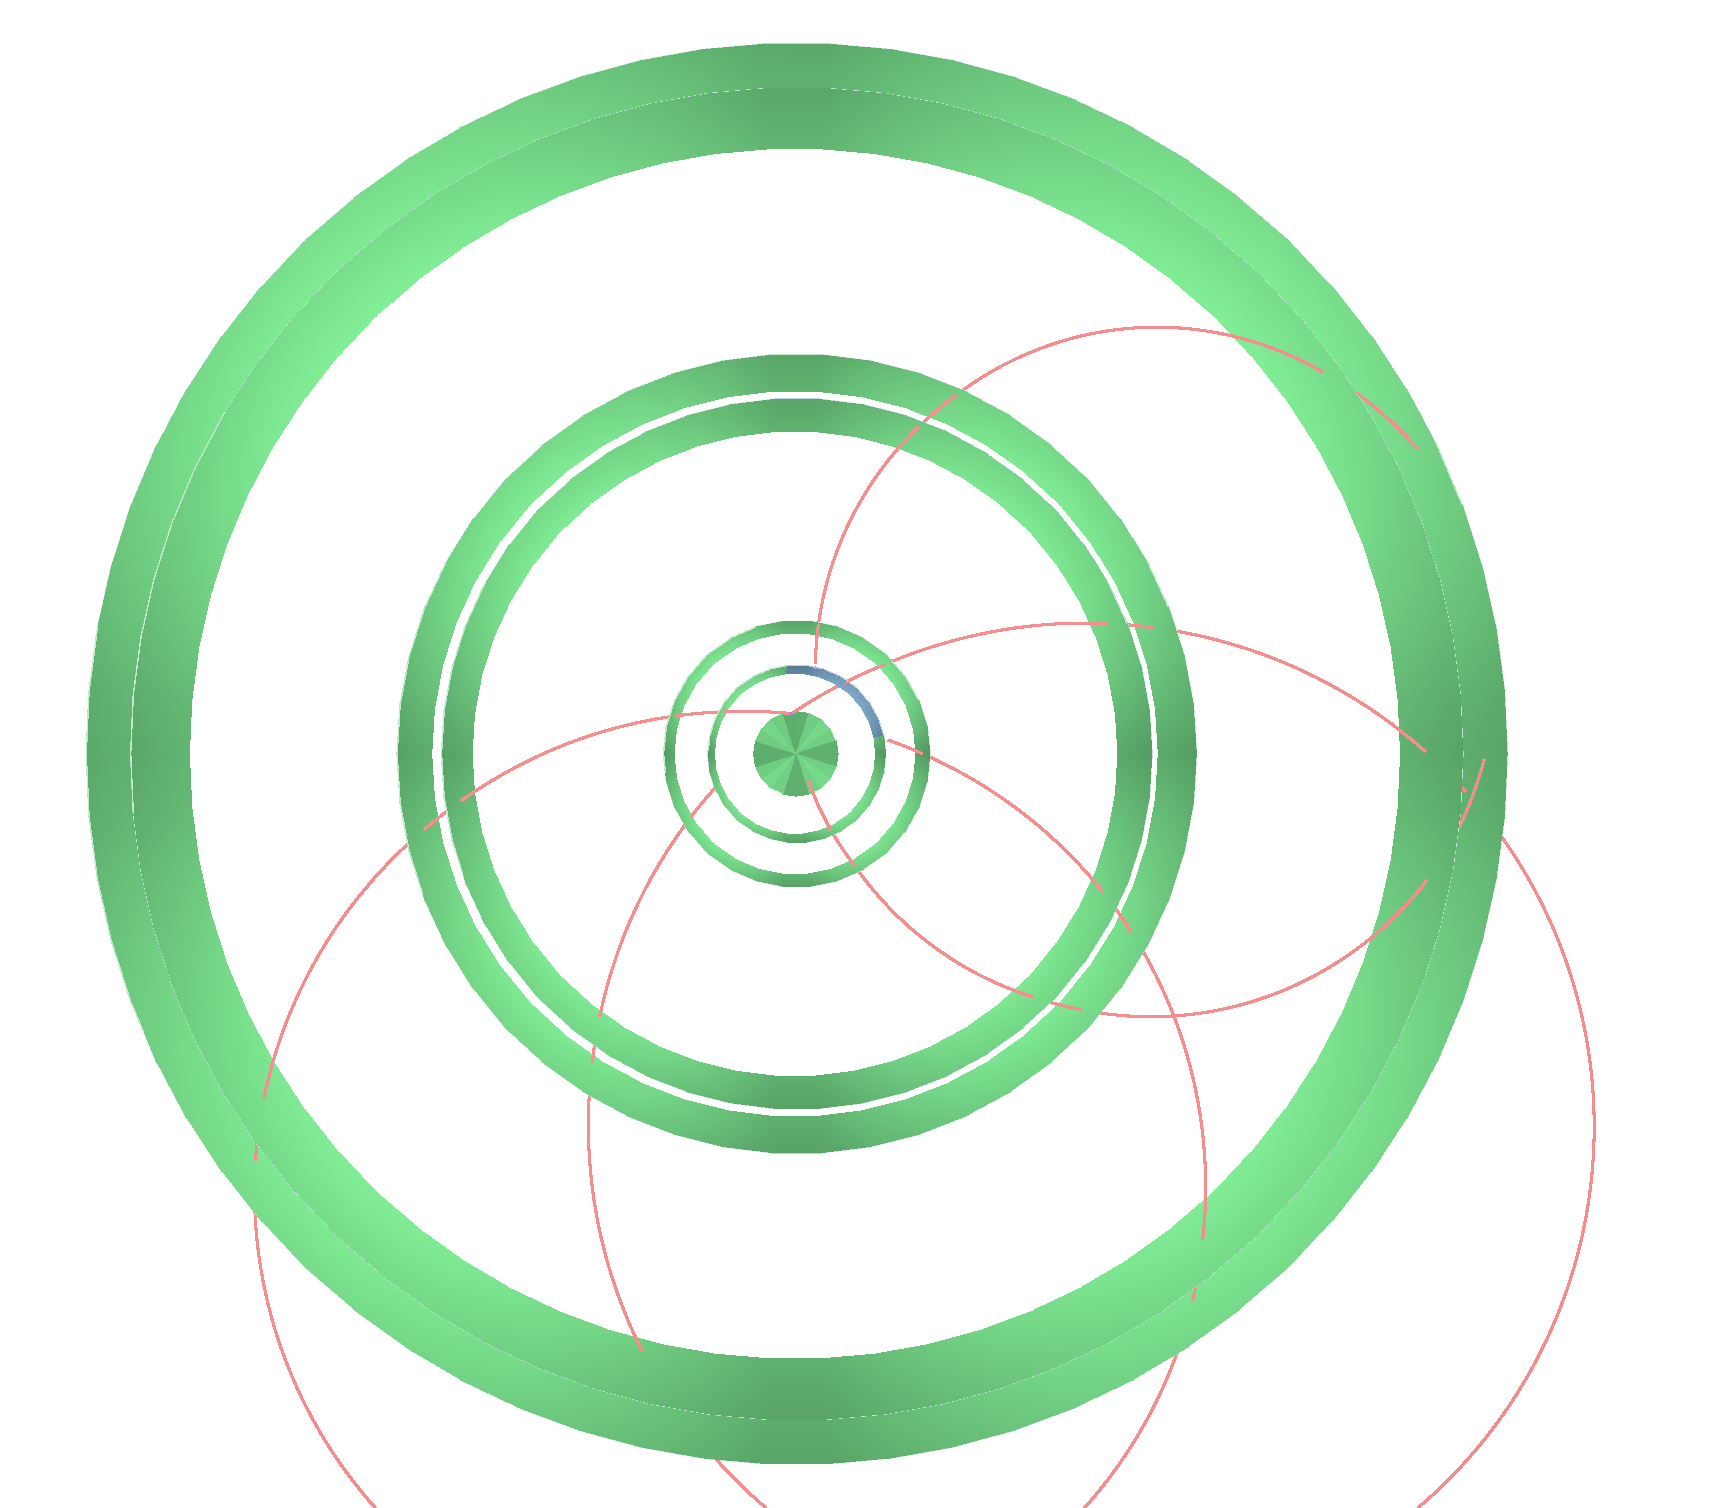
\includegraphics[width=\textwidth]{Figures/mu3e-evt0.pdf}
\end{center}
\endminipage\hfill
\minipage{0.55\textwidth}
\begin{center}
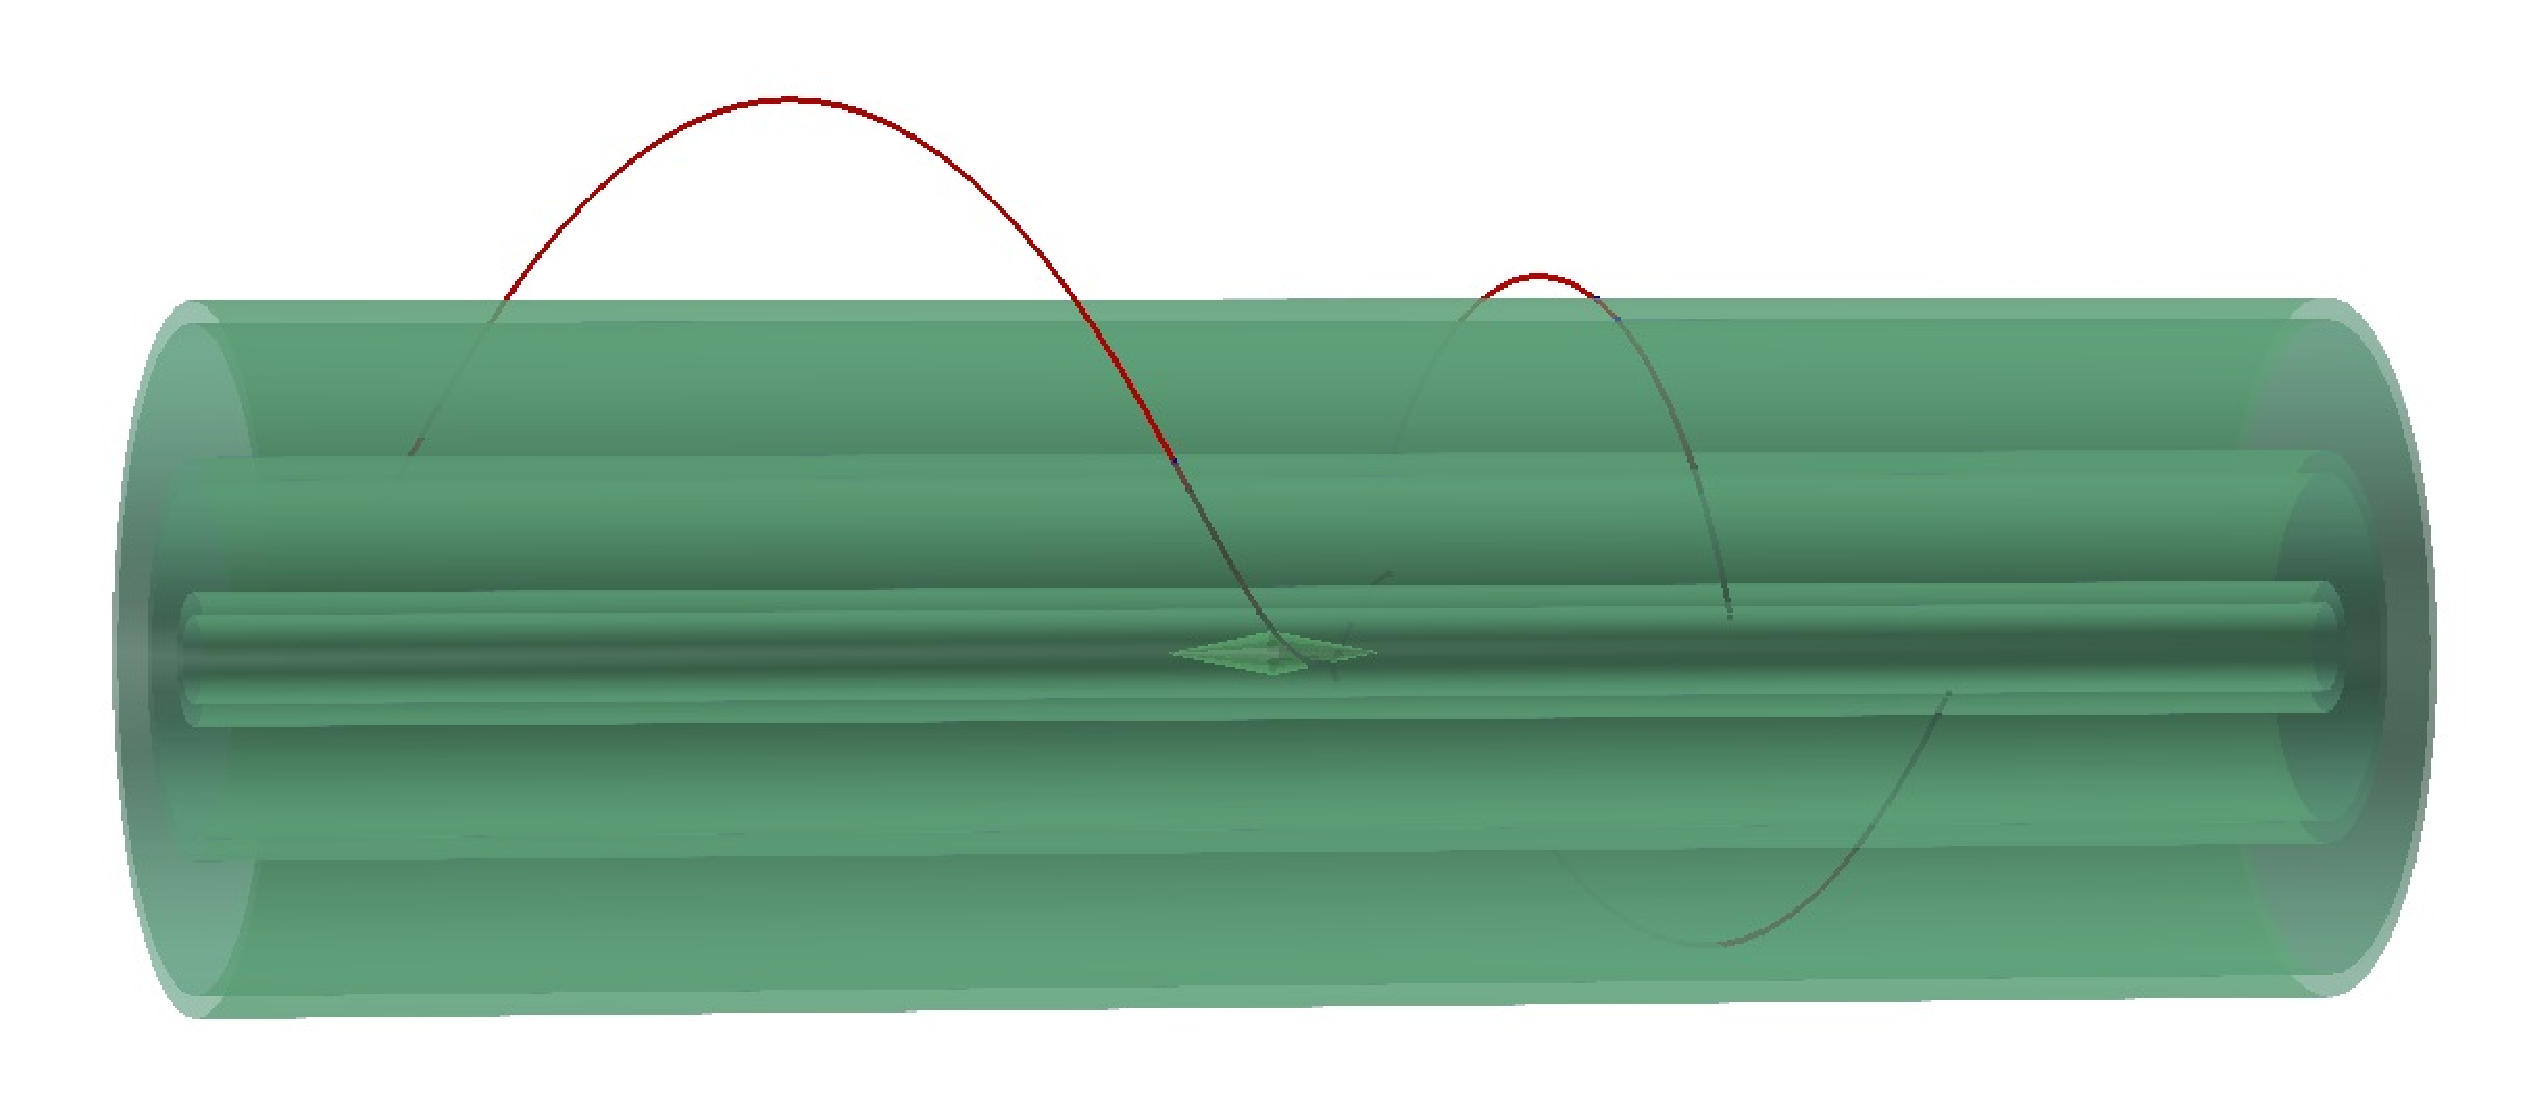
\includegraphics[width=\textwidth]{Figures/mu3e-evt1.pdf}
\end{center}
\vspace{0.5cm}
\endminipage\hfill
\caption{Display of the experimental setup, together with a simulated $\mu^+ \rightarrow e^+e^-e^+$ event.}
\label{Fig::mu3e}
\end{figure}

We generate $\mu^+ \rightarrow e^+e^-e^+$ events according to phase space to study the detector resolution and efficiency. The stopped muons are reconstructed by combining three electrons, constraining the tracks to originate from the same pixel in the active target. To further improve the resolution, we require the probability of the constrained fit to be greater than 1\%, and a reconstructed muon momentum less than $1 ~\Mev$. The absolute value of the cosine of the polar angle of each electron must also be less than 0.9. The resulting $e^+e^-e^+$ invariant mass distribution, shown in Fig.~\ref{Fig::mu3e2}, peaks sharply at the muon mass. We extract the resolution by fitting this spectrum with a double-sided Crystal Ball function (a Gaussian with power-law tails on both sides). The Gaussian resolution is found to be $0.3~\Mev$. To investigate the contribution of the active target to the resolution, we performed alternative fits, removing the geometric constraints, or taking the vertex position by considering all points from tracks intercepting the target, and choosing the one minimizing the $\chi^2$ of the constrained fit. While we observe an improvement compared to the unconstrained fit, the second method yields a similar signal resolution. However, the active target provides a better estimate of impact parameters of the tracks, improving background rejection.

\begin{figure}[htb]
\begin{center}
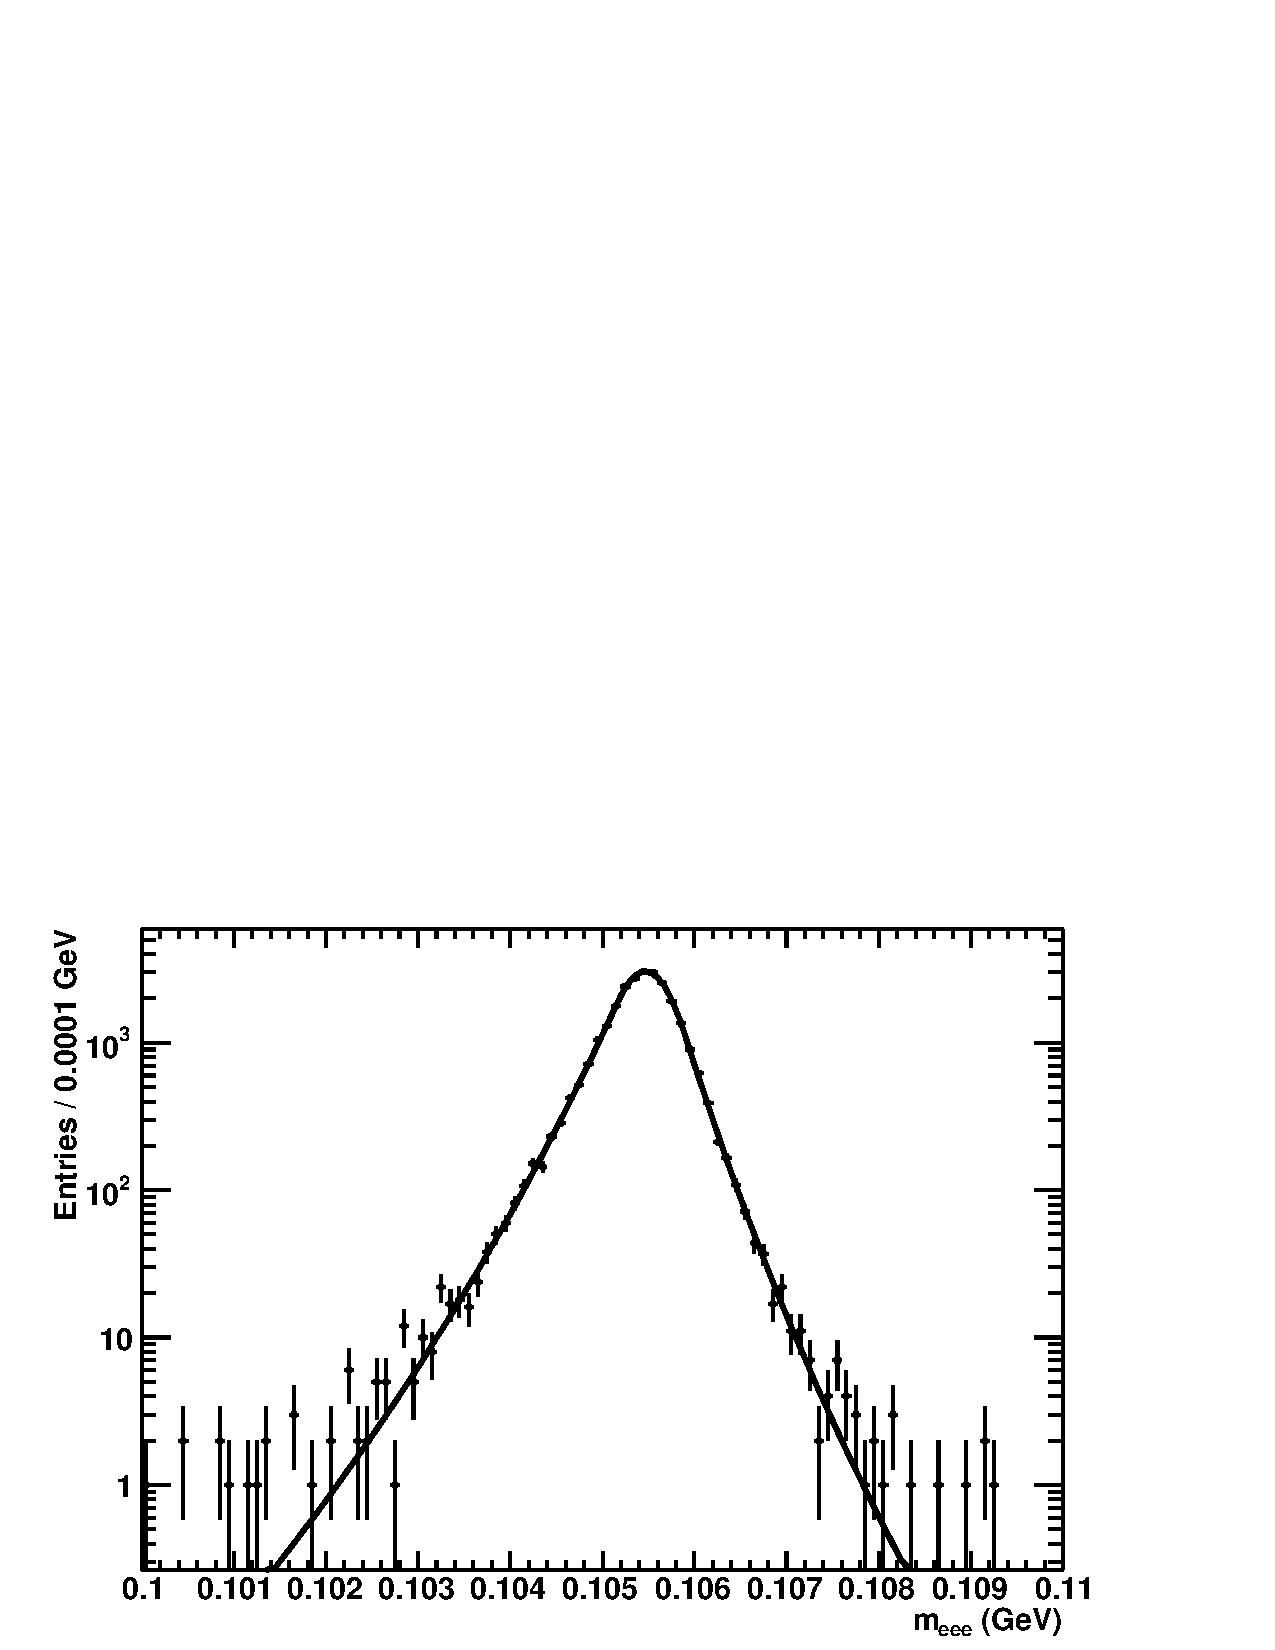
\includegraphics[width=0.6\textwidth]{Figures/mu3e-resoFit.pdf}
\end{center}
\caption{The $e^+e^-e^+$ invariant mass distribution after all selection criteria are applied fitted by a double-sided Crystal Ball function.}
\label{Fig::mu3e2}
\end{figure}

The signal efficiency is found to be 27\%. To achieve a SES at the level of $5\times\sim 10^{-18}$ after a 3-year run with 100\% DAQ efficiency, a stopped muon rate of the order of $8\times 10^{9}$ is needed. For comparison, the Mu3e stopped muon rate at the HiMB beam at PSI is expected to be of the order of $2\times 10^{9}$.   

To estimate the background contributions under these running conditions, we define a signal window as $ 104.9 < m_{eee} < 106.5 ~\Mev$, containing approximately 90\% of the signal. The irreducible background arises from $\mu \rightarrow e^+e^-e^+ \nu\bar\nu$ events where the two neutrinos carry almost no energy. We estimate its contribution to be about 8 events by convolving the branching fraction with the resolution function and integrating in the signal region, as shown in Figure~\ref{Fig::mu3e3}. However, this background depends strongly on the tail of the mass distribution, and small improvements translate into large background reductions. For example, decreasing the thickness of the silicon sensors and the supporting kapton structure by 20\% (40\%) reduces the background down to $\sim 4$ ($\sim 1$) events. Additional improvements of the reconstruction algorithms might further improve the resolution and reduce this contamination as well.

\begin{figure}[htb]
\begin{center}
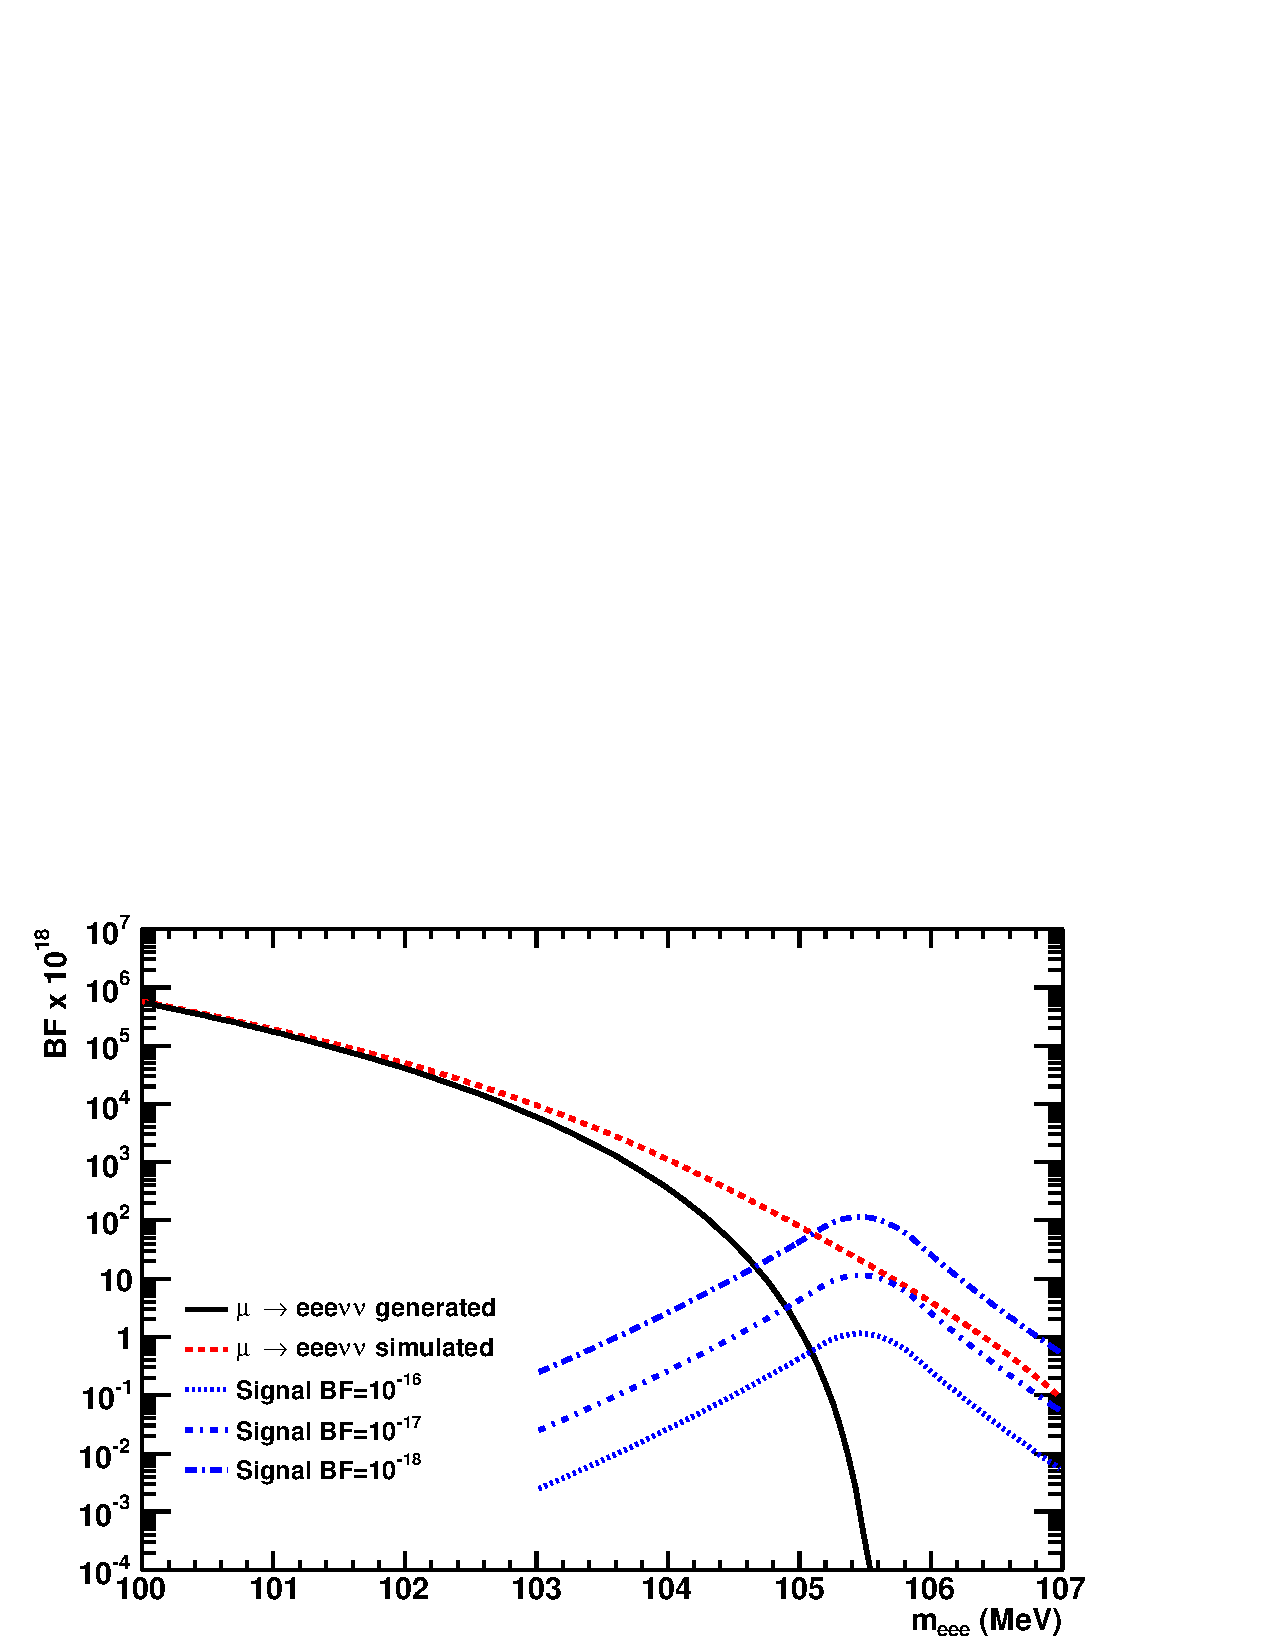
\includegraphics[width=0.45\textwidth]{Figures/mu3e-irr.pdf}
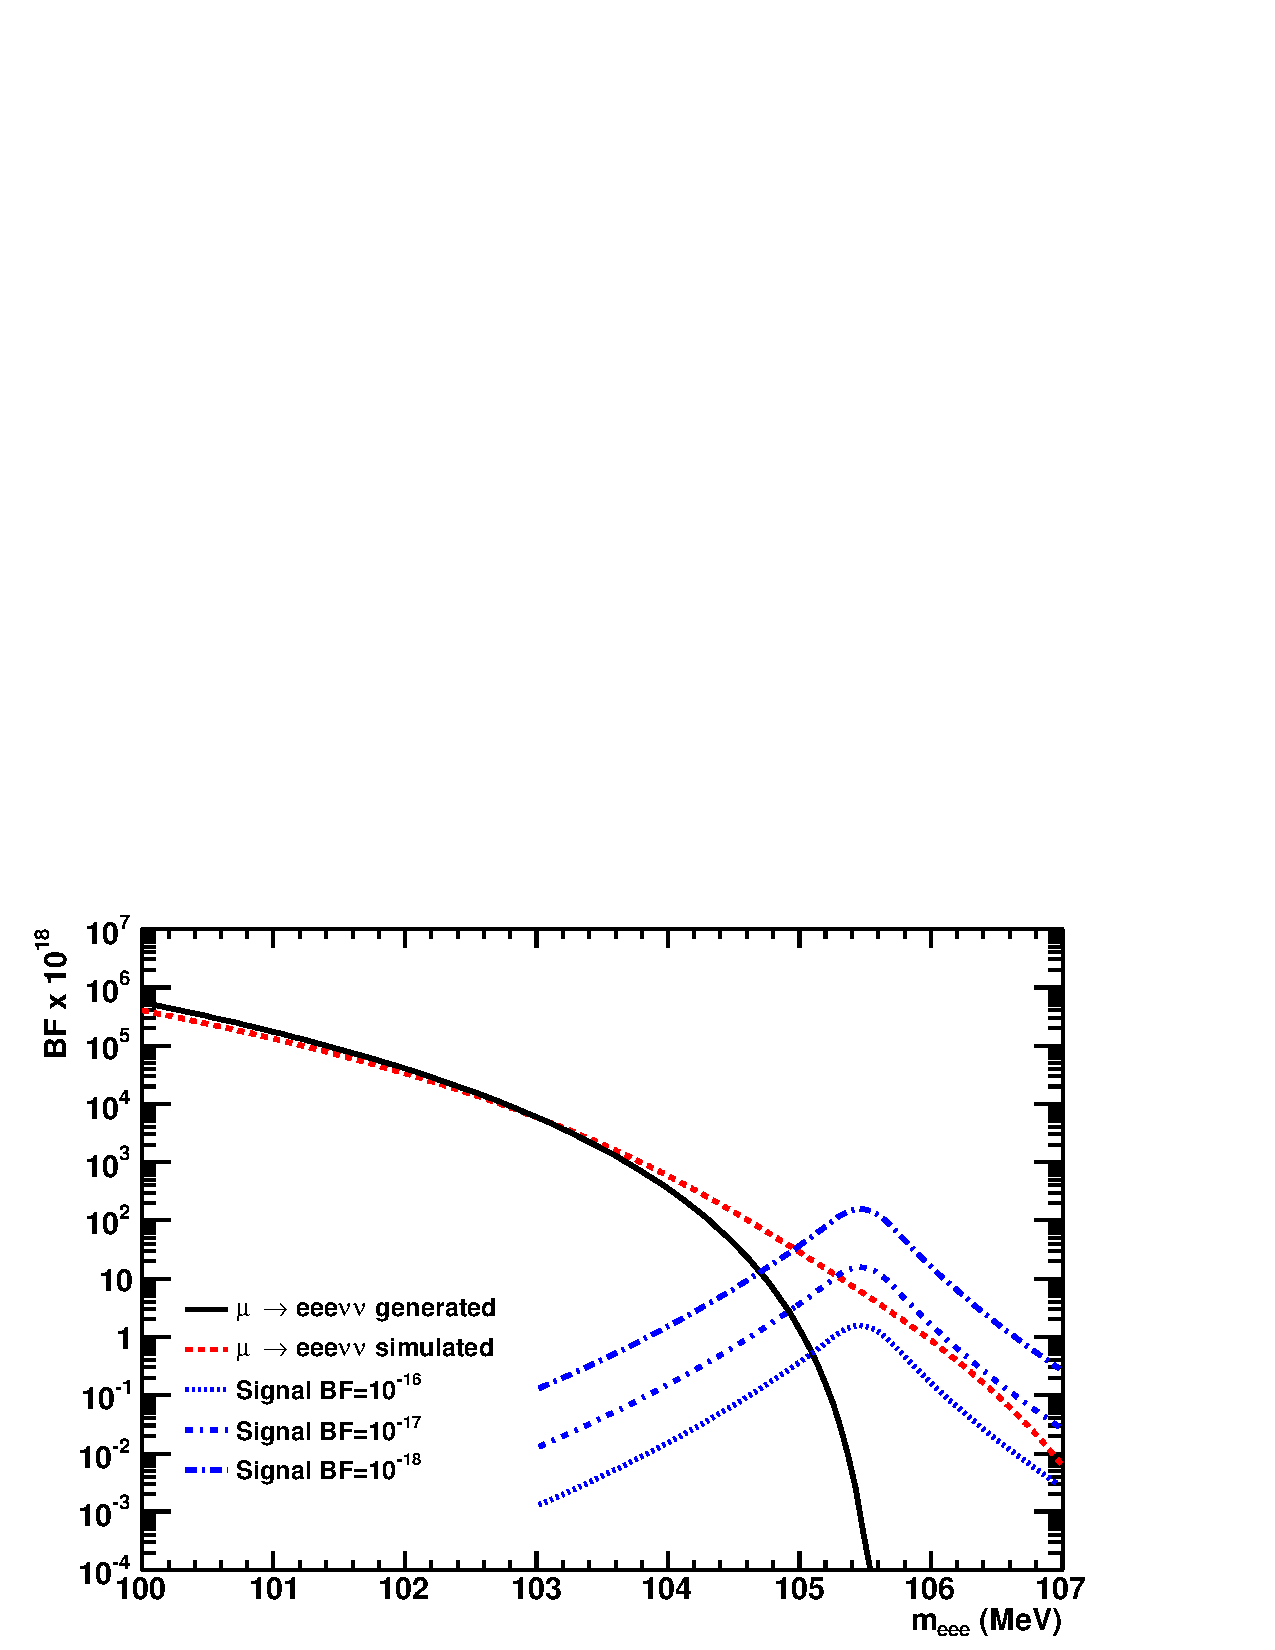
\includegraphics[width=0.45\textwidth]{Figures/mu3e-irr2.pdf}
\end{center}
\caption{The $\mu^+ \rightarrow e^+e^-e^+\nu_e \bar\nu_\mu$ branching fraction before and after convolution with the detector resolution overlaid with signal at different branching 
fractions. Results are shown for 50$\mu$m thick silicon sensors (left) and 30$\mu$m thick silicon sensors (right).}
\label{Fig::mu3e3}
\end{figure}

We consider accidental backgrounds produced by the combination of a Michel decay and a radiative Michel decay (2M$\gamma$ decays), or three simultaneous Michel decays (3M decays), where one of the the positrons is misreconstructed or produces an electron by interacting with the detector. In both cases, we assume the decays occurs within the same pixel in the active target, and during the same time window. This yields position and time suppression factors $\delta S = 7.8\times 10^{-7}$ and $\delta t = 2.5\times 10^{-10}$, respectively. The number of background events per second can be expressed as:
%
$$N_{2M\gamma} = {R_\mu}^2 \delta S \delta t {B(\mu^+ \rightarrow e^+ \nu_e \bar\nu_\mu)}^2 B(\mu^+ \rightarrow e^+ \nu_e \bar\nu_\mu \gamma) P(\gamma \rightarrow e^+ e^-)  P_\mu  \simeq 0.33 P_\mu$$
$$N_{3M} = {R_\mu}^3(\delta S)^2 {B(\mu^+ \rightarrow e^+ \nu_e \bar\nu_\mu)}^3 (\delta t)^2 P_\mu \simeq 0.02 P_\mu$$
%
where $P(\gamma \rightarrow e^+ e^-)\sim 0.18\%$ is the probability of photon conversion in the target and $P_\mu$ denotes the probability to reconstruct a muon candidate after all selection criteria are applied. The factors $P_\mu$ are estimated by Monte Carlo simulation using the matrix element and differential decay width given in Ref.~\cite{Kuno:1999jp,Djilkibaev:2008jy}. Values of $P_\mu$ of the order of ${\cal O}(10^{-8})$ (${\cal O}(10^{-9})$) are found for 2M$\gamma$ (3M) decays. Both backgrounds are estimated to be less than one event. A similar background level is expected from combinations of $\mu^+ \rightarrow e^+ \overline{\nu}_{\mu} \nu_e$ and $\mu^+ \rightarrow e^+e^-e^+ \overline{\nu}_{\mu} \nu_e$ decays. 

In summary, we have outlined the requirements needed to improve the projected sensitivity of the Mu3e experiment by an order of magnitude using a compact silicon tracker surrounding an active target. We estimate that a stopped muon rate of ${\cal O}(8\times 10^{9})$ would be required to achieve a SES of $5\times 10^{-18}$ for a 3-year run with 100\% DAQ efficiency. Relatively modest improvements on the resolution are needed to maintain the irreducible background at an appropriate level, while an active target proves to be essentially in the reduction of accidental backgrounds. 


